% SPDX-FileCopyrightText: 2026 林芳亘
% SPDX-FileCopyrightText: 2026 施嘉韙
% SPDX-FileCopyrightText: 2026 彭俊恆
% SPDX-FileCopyrightText: 2026 許芯瑀
% SPDX-FileCopyrightText: 2026 楊承軒
% SPDX-FileCopyrightText: 2026 高至言
% SPDX-FileCopyrightText: 2026 簡妤安
% SPDX-License-Identifier: Apache-2.0
\documentclass[11pt,a4paper]{article}
\usepackage[margin=2.4cm]{geometry}

% ============================================================================
% Compiler detection and font setup
% ============================================================================
% LuaLaTeX is required for Chinese/Japanese/Korean (CJK)) documents.
% XeLaTeX also works for CJK. pdfLaTeX supports Latin, Latin Extended,
% and Cyrillic scripts only.
%
% Font strategy:
%   CJK body: Noto Serif CJK TC (Taiwan MOE-conformant Ming/Song style)
%   CJK sans: Noto Sans CJK TC  (Taiwan MOE-conformant Hei/Gothic style)
%   CJK mono: Noto Sans Mono CJK TC
%   Latin:    Latin Modern (TeX Live bundled default)
%
% Install Noto CJK fonts (see Appendix B):
%   macOS:  brew install --cask font-noto-serif-cjk-tc font-noto-sans-cjk-tc
%   font-noto-sans-mono-cjk-tc
%   Linux:  apt install fonts-noto-cjk fonts-noto-cjk-extra  (or distro equivalent)
%   Windows: download from https://fonts.google.com/noto
\usepackage{iftex}
\ifluatex
    % ── LuaLaTeX ─────────────────────────────────────────────────────────
    \usepackage{fontspec}
    % scheme=plain: load CJK font support without redefining \abstractname,
    % \today, or section names to Chinese (keeps English/ISO defaults).
    % fontset=none: avoid ctex auto-detecting macold fontset on modern macOS
    % (STHeiti/STKaiti/STFangsong removed since macOS 10.12).
    \usepackage[scheme=plain,fontset=none]{ctex}
    \setCJKmainfont{Noto Serif CJK TC}
    \setCJKsansfont{Noto Sans CJK TC}
    \setCJKmonofont{Noto Sans Mono CJK TC}
\else\ifxetex
    % ── XeLaTeX ──────────────────────────────────────────────────────────
    \usepackage{fontspec}
    \usepackage{xeCJK}
    \setCJKmainfont{Noto Serif CJK TC}
    \setCJKsansfont{Noto Sans CJK TC}
    \setCJKmonofont{Noto Sans Mono CJK TC}
\else
    % ── pdfLaTeX ─────────────────────────────────────────────────────────
    % T1 encoding for correct hyphenation of latin scripts:
    %   - All Western European (English, French, German, Spanish, Italian, etc.)
    %   - All Nordic/Scandinavian (Swedish, Finnish, Danish, Norwegian, Icelandic)
    %   - Central/Eastern European (Polish, Czech, Slovak, Hungarian, Romanian,
    %     Croatian, Slovenian, Estonian, Latvian, Lithuanian,Turkish)
    %   - Other Latin-script languages (Vietnamese with VNTeX, Esperanto, etc.)
    \usepackage[T1]{fontenc}
    % Scalable Latin Modern, which fontspec loads by default under the
    % other two engines.
    \usepackage{lmodern}
    % Unlike the LaTeX template, this report keeps pdfLaTeX's error on a CJK
    % character: a character dropped silently would go unnoticed in a
    % submitted report. Use LuaLaTeX to render CJK text (Appendix B).
\fi\fi

% ============================================================================
% Common packages (work with all compilers)
% ============================================================================
\usepackage{amsmath,amssymb,amsthm}
\usepackage{graphicx}
\usepackage{xcolor}
\usepackage[colorlinks=true,linkcolor=blue!70!black,citecolor=green!50!black,urlcolor=blue!70!black]{hyperref}
\usepackage{booktabs}
\usepackage{float,caption}
\captionsetup{font=small,labelfont=bf}
\setlength{\parskip}{3pt}
% Additions for this report:
\usepackage{microtype}  % Better line breaking
\usepackage{csquotes}   % Quotation marks, which biblatex-apa expects
\usepackage{siunitx}    % Numbers and units: \num, \qty, \unit
\usepackage{listings}   % Code listings
\lstset{basicstyle=\ttfamily\small, frame=single, columns=fullflexible,
  breaklines=true}

% ============================================================================
% Bibliography backend — biblatex + biber, APA 7th edition (author-year)
% ============================================================================
% references.bib uses the biblatex format, which biber reads; bibtex would
% fail on it, so cite with \textcite and \parencite. annotation=false keeps
% private notes in the annote field of an entry out of the reference list,
% which biblatex-apa would otherwise print.
\usepackage[backend=biber,style=apa,natbib=true,
            annotation=false]{biblatex}
\addbibresource{references.bib}

% Graphics path
\graphicspath{{figures/}}

% Hyperref setup: the title and authors stored in the PDF file
\hypersetup{
    pdftitle={Experimental Characterization of Duckiebot Wheel Dynamics},
    pdfauthor={林芳亘, 施嘉韙, 彭俊恆, 許芯瑀, 楊承軒, 高至言, 簡妤安},
}

% cleveref must be loaded after hyperref (addition for this report).
\usepackage[capitalise,noabbrev]{cleveref}

% ISO date format (YYYY-MM-DD)
\usepackage[style=iso]{datetime2}

% ============================================================================
% Document metadata
% ============================================================================
\title{Experimental Characterization of Duckiebot Wheel Dynamics}
\author{\setlength{\tabcolsep}{4pt}\begin{tabular}{ccccccc}
林芳亘 & 施嘉韙 & 彭俊恆 & 許芯瑀 & 楊承軒 & 高至言 & 簡妤安 \\
\footnotesize E14131639 & \footnotesize E14131906 & \footnotesize E14135015 & \footnotesize E14136338 & \footnotesize E14136508 & \footnotesize E14136574 & \footnotesize E14131207
\end{tabular}}
\date{\small Group 03, Department of Mechanical Engineering, National Cheng Kung University, Taiwan\\ Automatic Control -- Experiment 2\\ 2026-11-26}

\begin{document}
\maketitle
\begin{abstract}
This experiment investigated whether a linear first-order model describes the rotational dynamics of two Duckiebot wheel motors. Small-duty sweeps and repeated large-duty steps were recorded on a stand and processed using the course video-tracking and synchronization pipeline. The quality reports identified substantial disagreements between timing estimates and implausible angular velocities. For the right wheel, the automatically calculated rest-speed threshold was 41.50 rad/s, preventing the standard start-duty calculation and consequently the standard figure-generation workflow. Diagnostic analysis of the left wheel's available sweep showed an apparent onset near a duty magnitude of 0.28 and near-rest behavior near 0.22, but the timing alignment was not independently validated. Right-wheel step fits produced inconsistent gains and time constants, and the nominal rest intervals of two repetitions contained substantial apparent motion. These observations prevent reliable identification of motor parameters or quantitative verification of hysteresis. The results distinguish apparent nonlinear behavior from measurement artifacts and identify synchronization and tracking validation as prerequisites for a defensible controller model. The original measurements were retained without imputing the missing left-wheel forward sweep.
\end{abstract}
\noindent\textbf{Keywords:} wheel dynamics; system identification; dead zone; hysteresis; measurement quality
\section{Introduction}
The objective was to test three predictions of a linear motor model: response to small inputs (P1), invariance of gain and time constant with operating point (P2), and symmetry of increasing and decreasing inputs (P3). The experimental procedure and analysis follow the course repository \parencite{course}. This report distinguishes diagnostic calculations from validated physical estimates.
\section{Theory}
For duty input $u$ and angular velocity $\omega$, a first-order linear model is
\begin{equation}\tau\dot\omega+\omega=Ku.\end{equation}
For a step $\Delta u$ from equilibrium, the response is $\omega(t)=\omega_0+K\Delta u(1-e^{-t/\tau})$. A linear model predicts proportional steady-state changes, identical parameters at different operating points, and sign-reversed responses to opposite steps of equal magnitude. Static friction may cause a dead zone and different starting and stopping duties; however, timing or tracking errors can mimic these effects.
\section{Method}
The R3 robot was tested on a stand with left motor M5 and right motor M6. E1 used duty magnitudes from 0.10 to 0.36 in increments of 0.02; E2 used three repetitions of the schedule $0\to0.6\to1.0\to0.6\to0$. The phone recorded 1920 by 1080 pixels at nominally 240 frames/s; the actual rate was approximately 145 frames/s. All four videos used the same cyan-marker rule, \texttt{b>120 \& b-r>60 \& b-g>15}. Angular position and speed were obtained with the course tracking and processing scripts, with command logs aligned using light-emitting diode (LED) events or motion. The left forward-direction E1 trial was not recorded; no replacement was imputed. The available left negative-duty trial contains rising and falling duty magnitudes.

Both motor folders were processed and checked using the original course scripts. The standard plotting script failed during the StartDuty calculation. Diagnostic plots and independent step fits were therefore generated from processed data without changing raw logs or frame tables. Plateau means and standard deviations describe the aligned samples, not confidence intervals. The diagnostic calculations do not replace the official quality checks.
\section{Results}
\subsection{Data quality and rest noise (4e)}
Both quality reports warn against using the data as-is. Right E1 LED timing uncertainty was 85 ms, exceeding 10 ms; median motion-to-LED disagreement was 21.5 s. Left E1 used motion alignment after only 10 of 54 LED edges matched. Its trial-motion versus run-motion discrepancy was 19.6 s. For E2, the angle uncertainty scale factors were 204 (left) and 283 (right). Right E2 repetitions showed 16.5, 18.1 and 38.5\% of steady frames turning against duty, respectively. The third repetition also had 6.63\% of usable frames above 50 rad/s.
\begin{table}[H]\centering\caption{Right-wheel nominal rest intervals (rad/s). P99 is the 99th percentile of absolute speed.}\begin{tabular}{lrrr}\toprule Trial & Mean & SD & P99\\\midrule E1 backward & 0.013 & 0.784 & 1.809\\ E2 rep. 1 & -0.013 & 0.308 & 0.935\\ E2 rep. 2 & 5.991 & 6.203 & 17.509\\ E2 rep. 3 & 7.949 & 17.145 & 46.322\\\bottomrule\end{tabular}\end{table}
The official pooled threshold was 41.50 rad/s, larger than the expected 15--20 rad/s step speed in the course instructions. The first two listed intervals were much quieter than repetitions 2 and 3. The latter cannot be treated as stationary sensor noise without confirming their timing. No valid forward E1 rest samples were available. Excluding the two contaminated intervals diagnostically gives approximately 1.77 rad/s, but this is not an approved replacement threshold.
\begin{figure}[H]\centering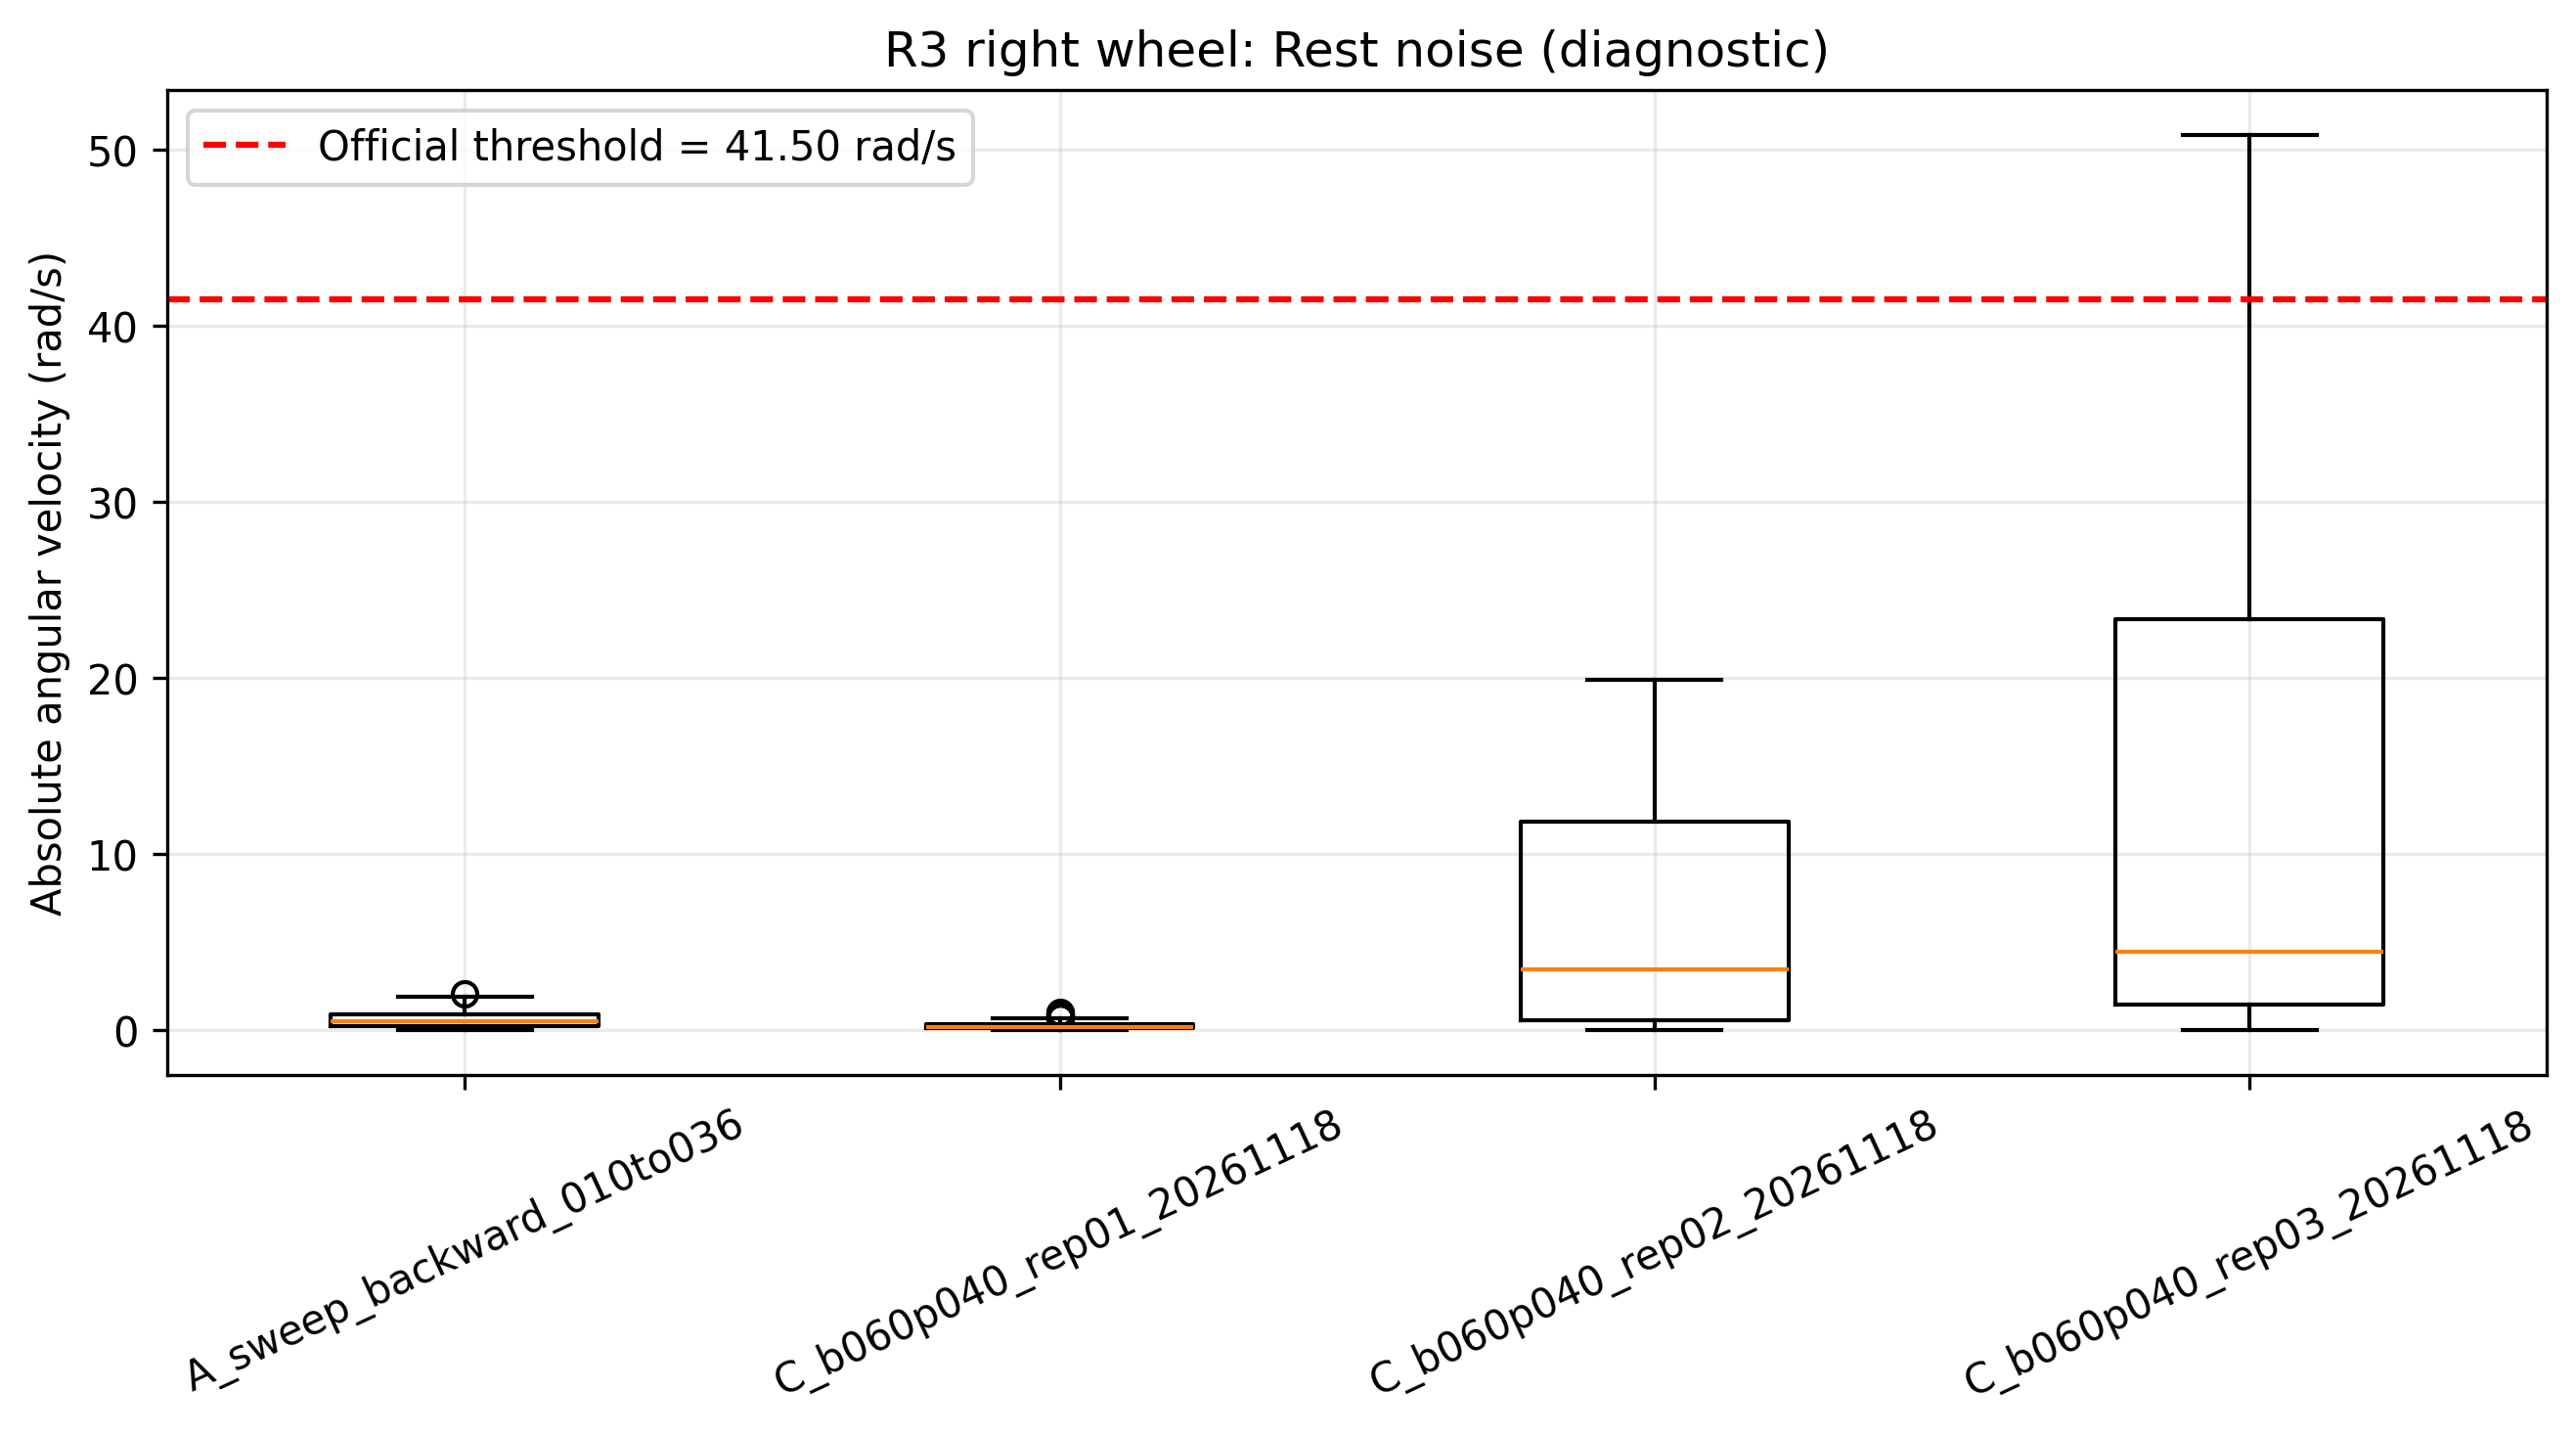
\includegraphics[width=0.85\linewidth,height=0.32\textheight,keepaspectratio]{R3_rest_noise_diagnostic.png}\caption{Nominal rest-speed noise, right wheel. Diagnostic plot; timing and tracking are not validated.}\end{figure}
\subsection{Small-duty response (4a, P1)}
The right forward sweep had rising plateau means with absolute magnitude no greater than 0.139 rad/s, below even the diagnostic threshold. The official StartDuty computation failed, so a validated start duty could not be reported. The left negative-duty sweep showed apparent onset at magnitude 0.28 (mean $-5.14$ rad/s), increasing to $-9.56$ rad/s at 0.32. This resembles a dead zone but the motion-based clock is uncertain; P1 cannot be conclusively tested.
\begin{figure}[H]\centering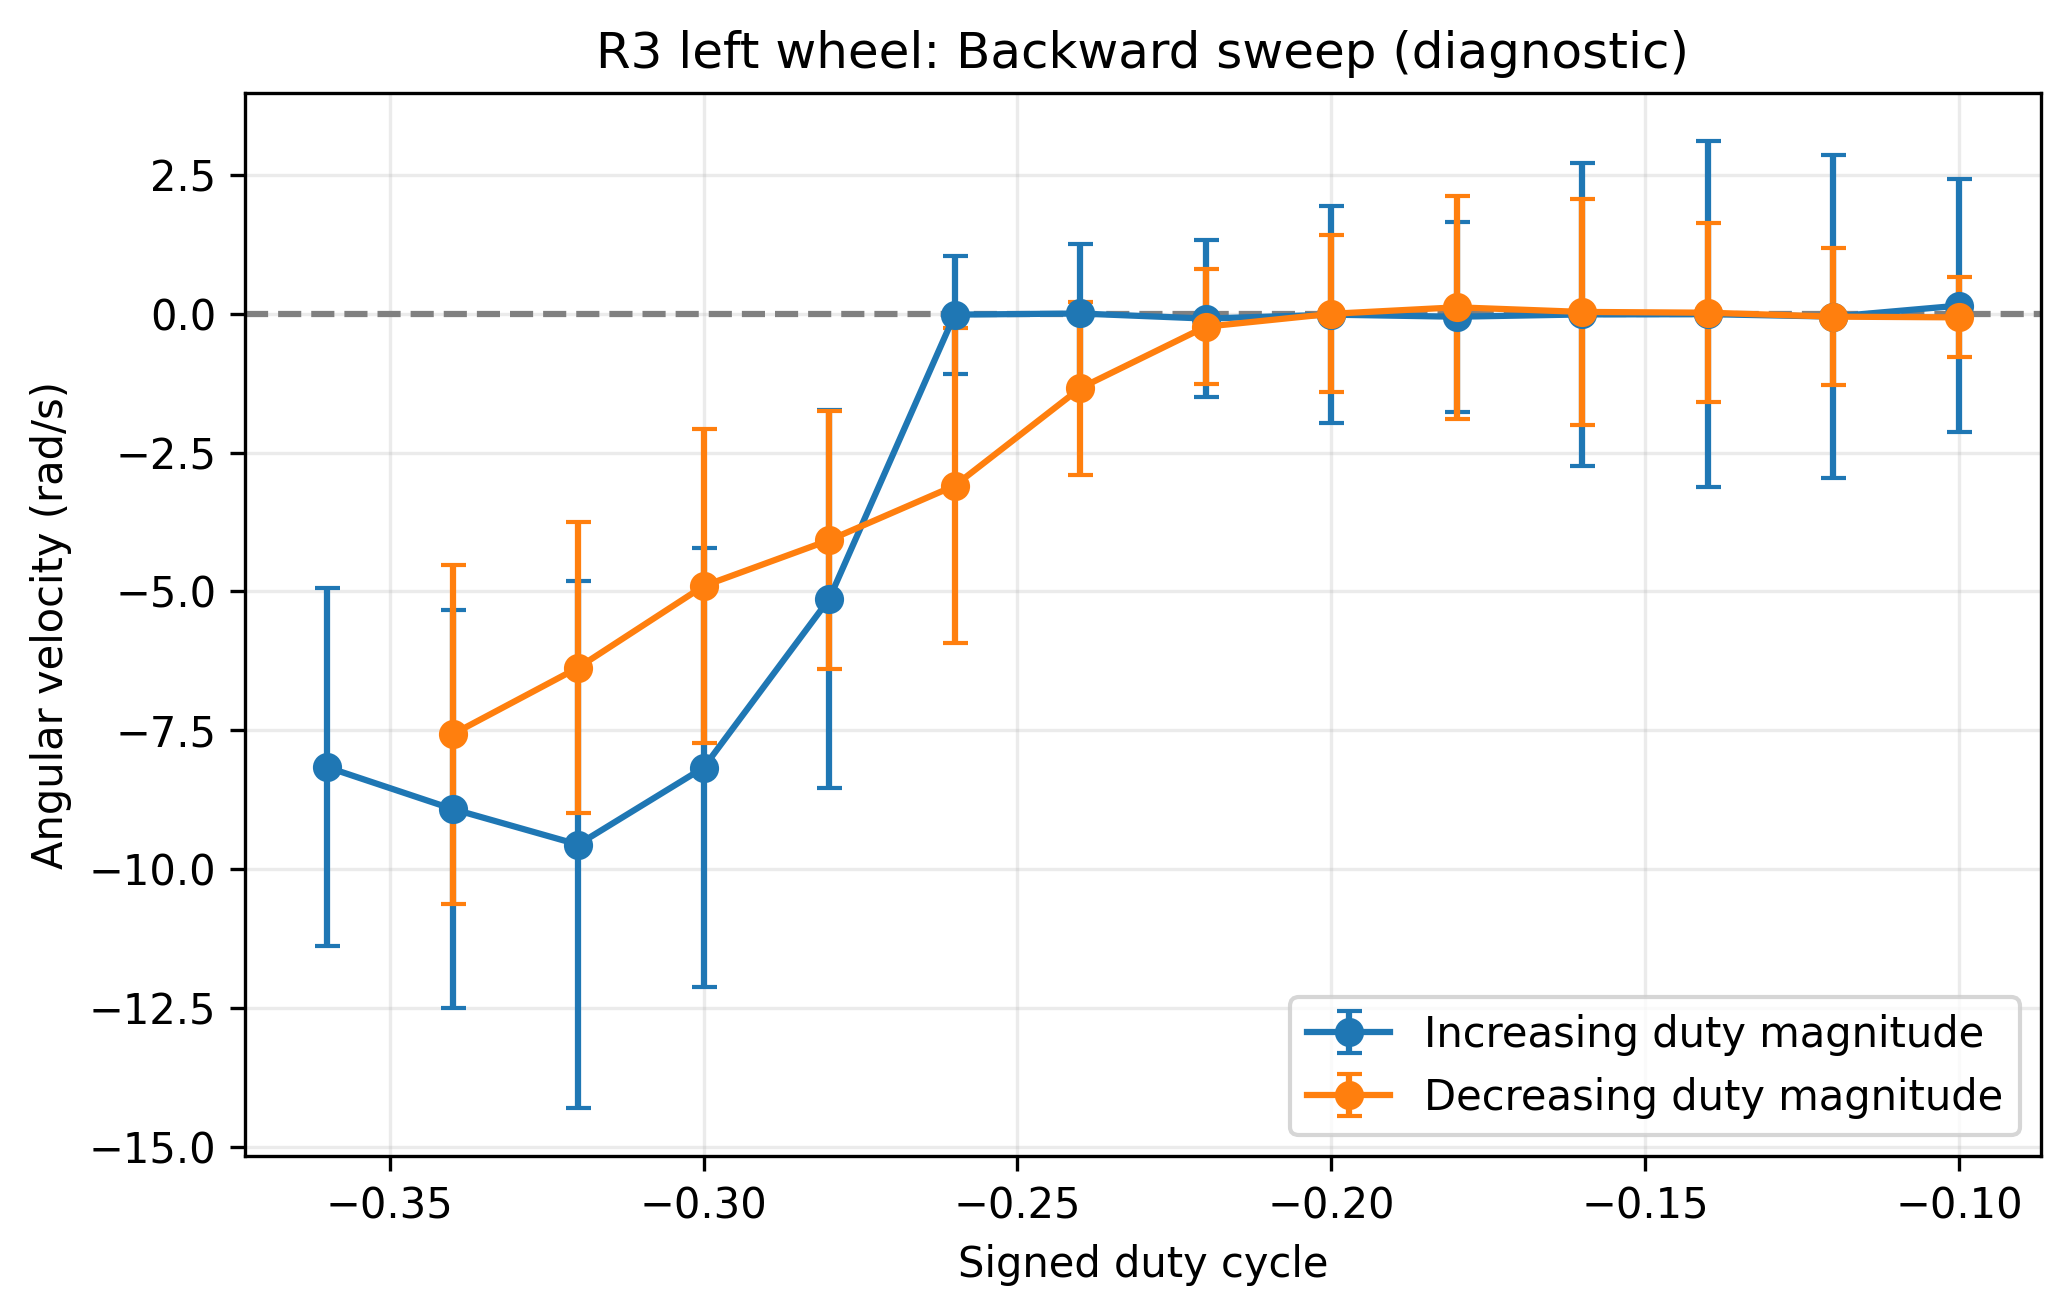
\includegraphics[width=0.85\linewidth,height=0.32\textheight,keepaspectratio]{R3_left_E1_backward_diagnostic.png}\caption{Left wheel, available negative-duty E1 branches. Diagnostic plot; timing and tracking are not validated.}\end{figure}
\subsection{Step response and operating point (4b--4c, P2)}
Independent diagnostic fits gave the values in Table~\ref{tab:fits}. The 0-to-0.6 step had almost no measured change in the aligned endpoint means, whereas the 0.6-to-1.0 step appeared to start near rest. The fitted gain for the first step would predict approximately $-0.023$ rad/s at duty 0.2, but this is not a valid physical prediction. The fit parameters differ strongly, yet the poor alignment and residuals prevent attributing the difference to operating-point dependence. Rise, overshoot and settling metrics were unavailable.
\begin{table}[H]\centering\caption{Diagnostic first-order fits; not validated motor parameters. Gain in rad/s per unit duty, time constant in seconds.}\label{tab:fits}\begin{tabular}{lrrr}\toprule Step & $K$ & $\tau$ & Relative RMS\\\midrule $0\to0.6$ & -0.116 & 0.056 & 22.76\\ $0.6\to1$ & 26.465 & 0.152 & 1.43\\ $1\to0.6$ & -31.439 & 0.063 & 1.84\\ $0.6\to0$ & 17.467 & 0.159 & 1.64\\\bottomrule\end{tabular}\end{table}
\begin{figure}[H]\centering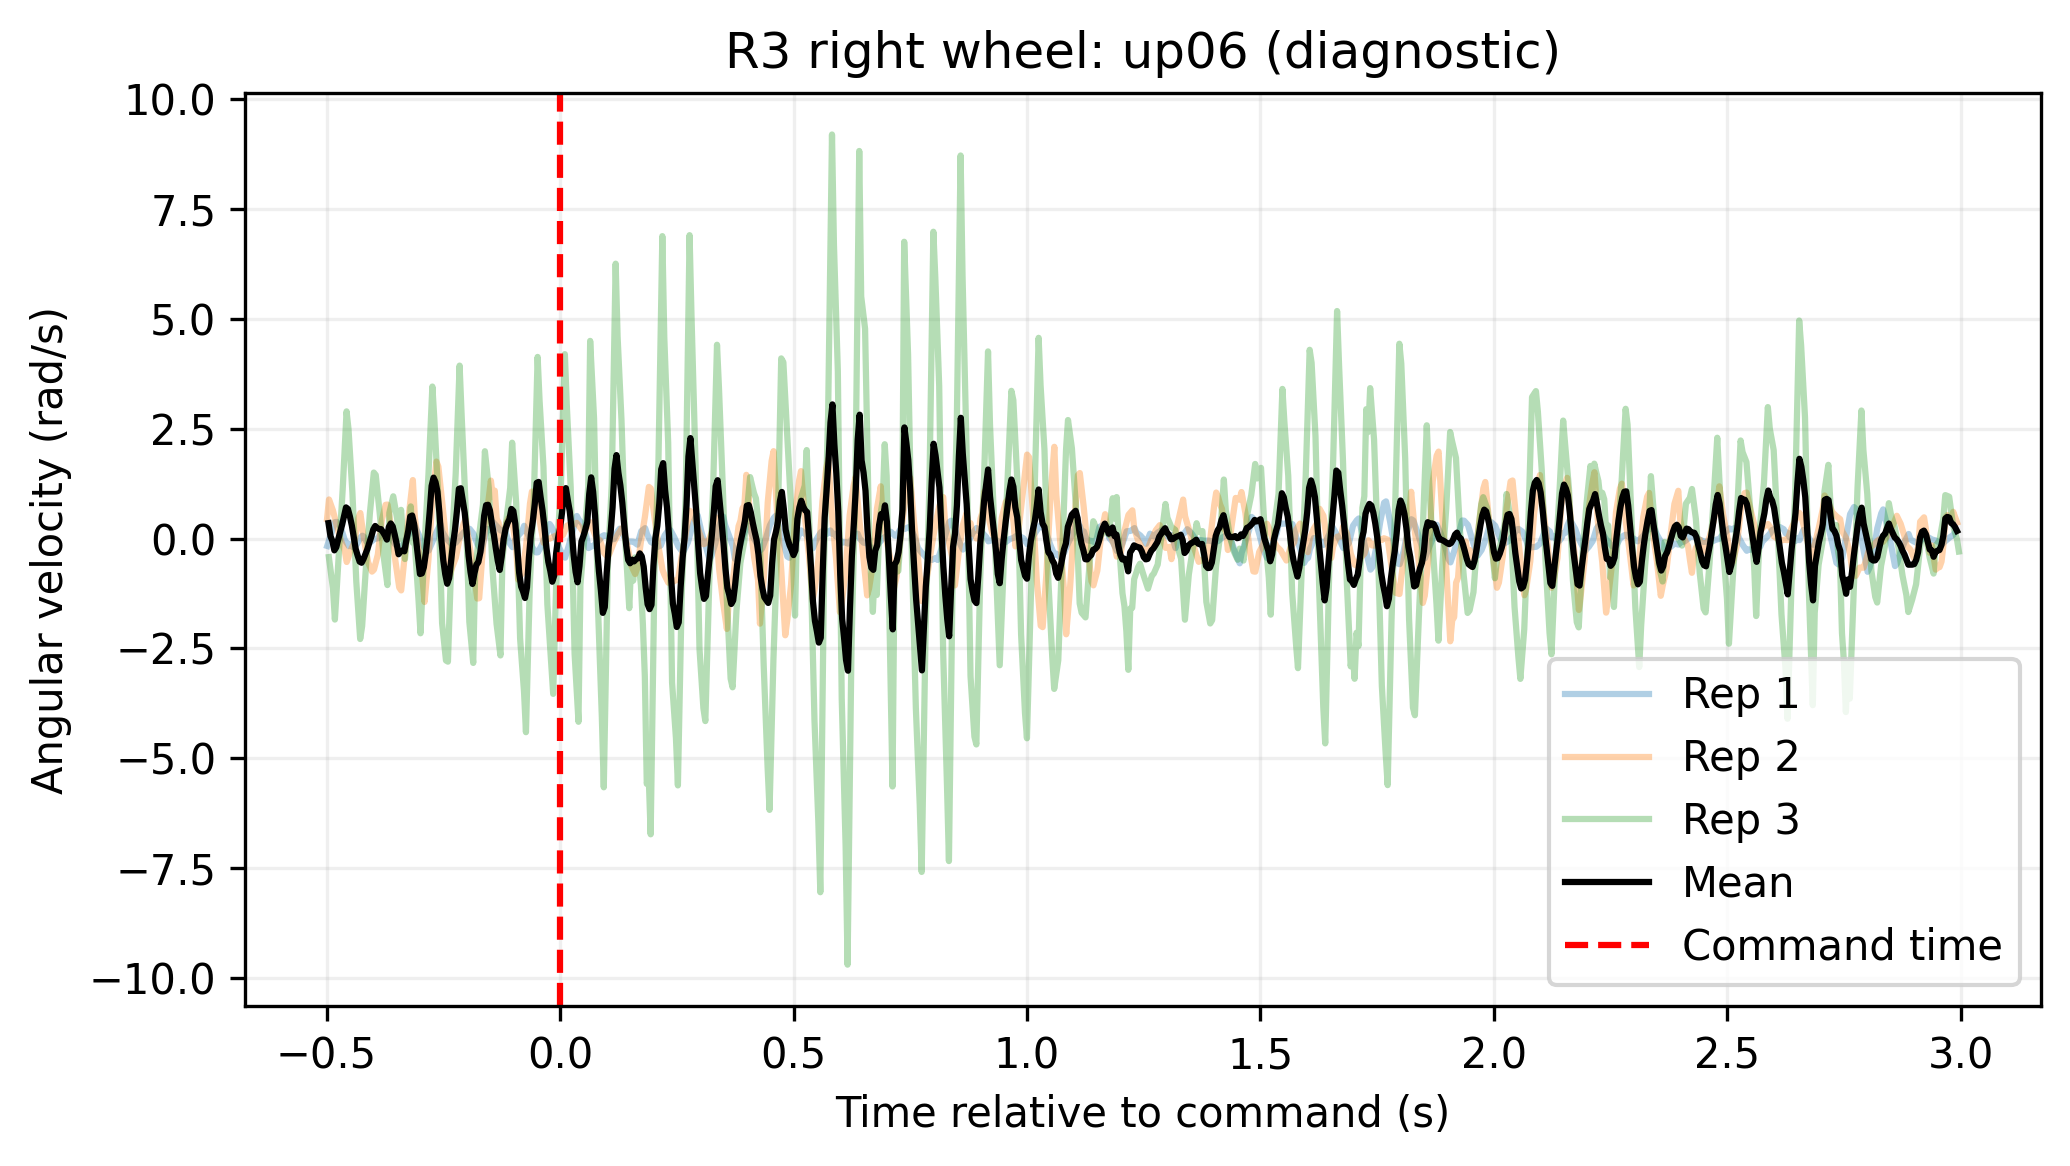
\includegraphics[width=0.85\linewidth,height=0.32\textheight,keepaspectratio]{R3_E2_up06_diagnostic.png}\caption{Right wheel, step from 0 to 0.6. Diagnostic plot; timing and tracking are not validated.}\end{figure}
\begin{figure}[H]\centering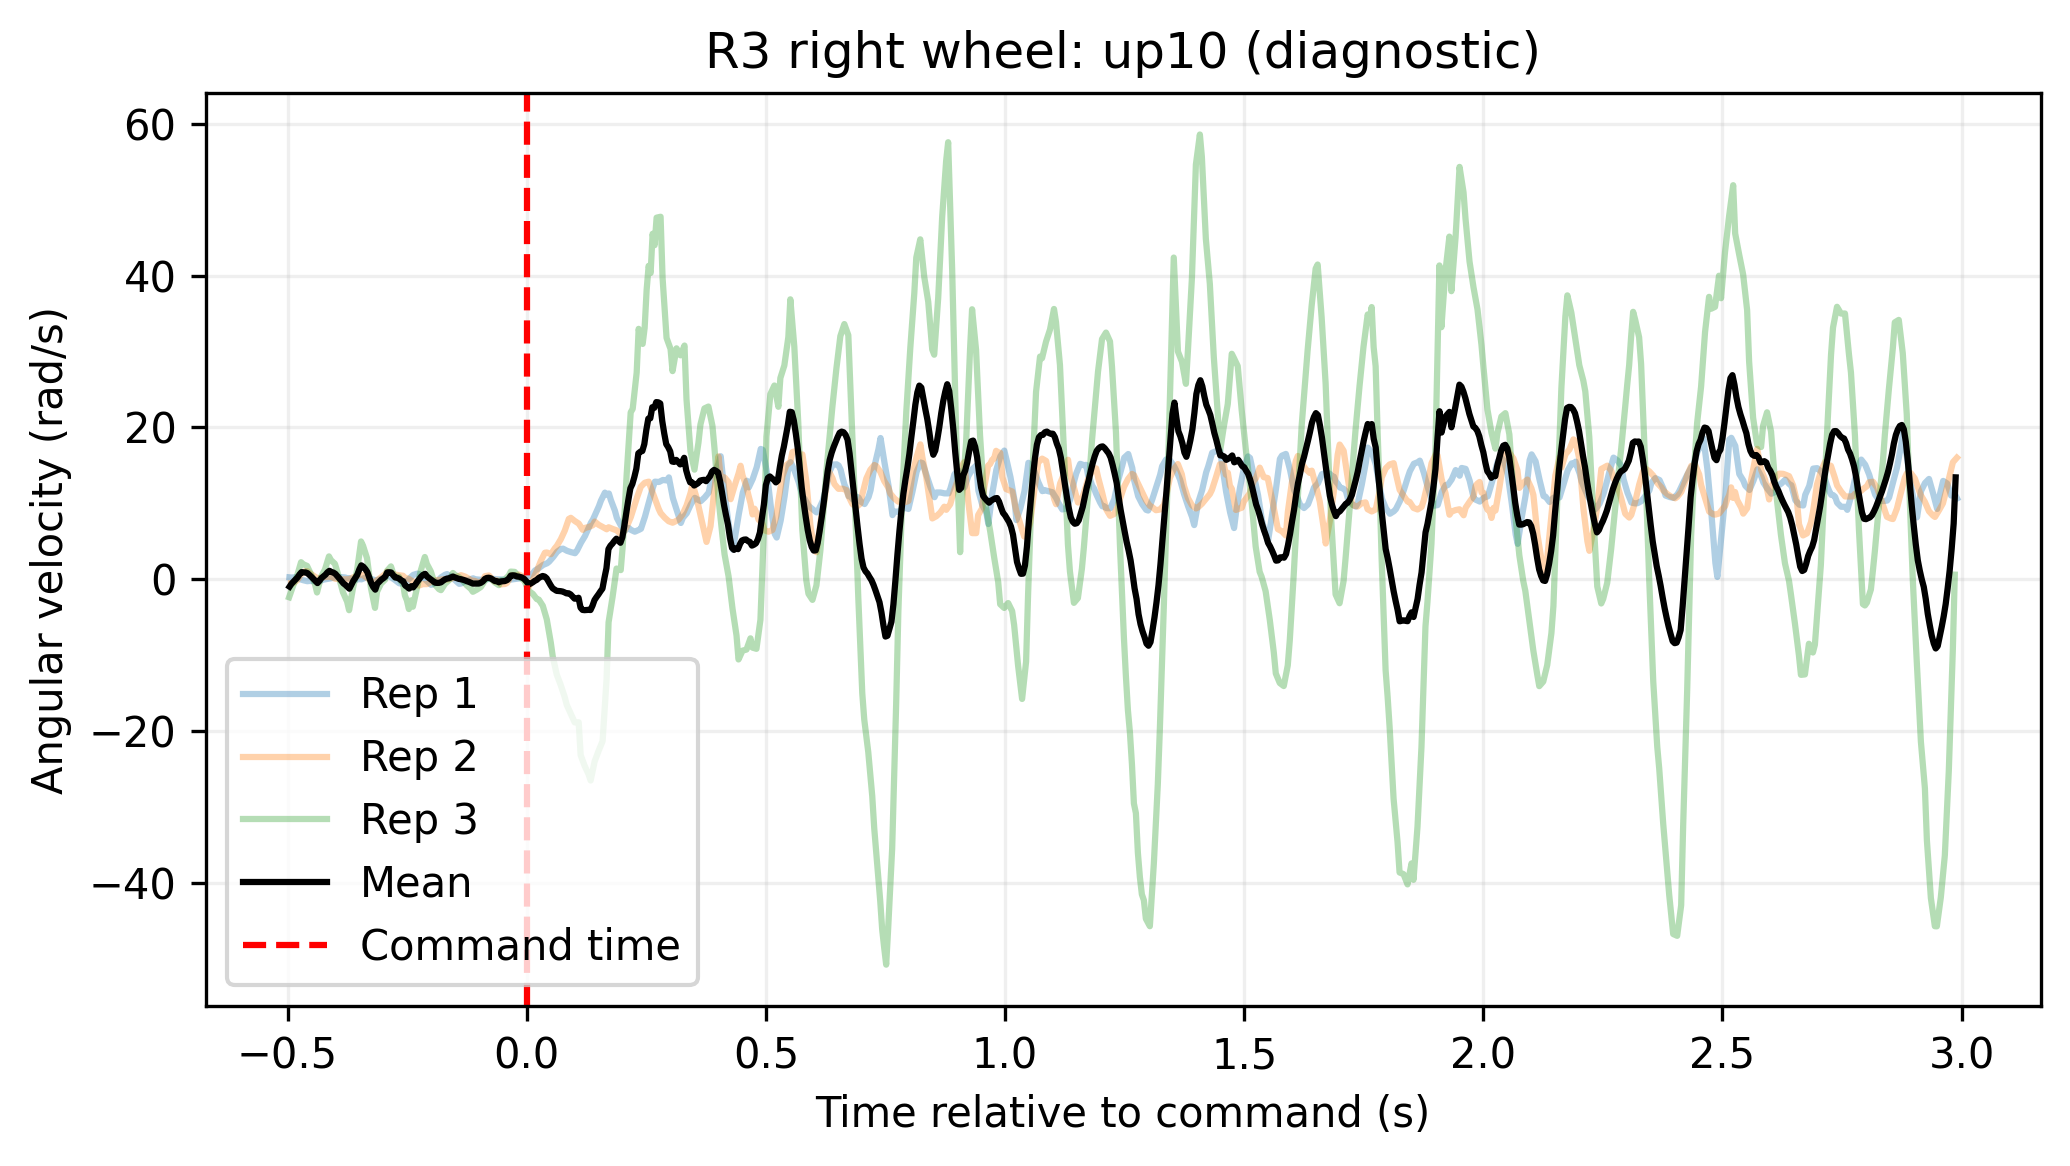
\includegraphics[width=0.85\linewidth,height=0.32\textheight,keepaspectratio]{R3_E2_up10_diagnostic.png}\caption{Right wheel, step from 0.6 to 1.0. Diagnostic plot; timing and tracking are not validated.}\end{figure}
\begin{figure}[H]\centering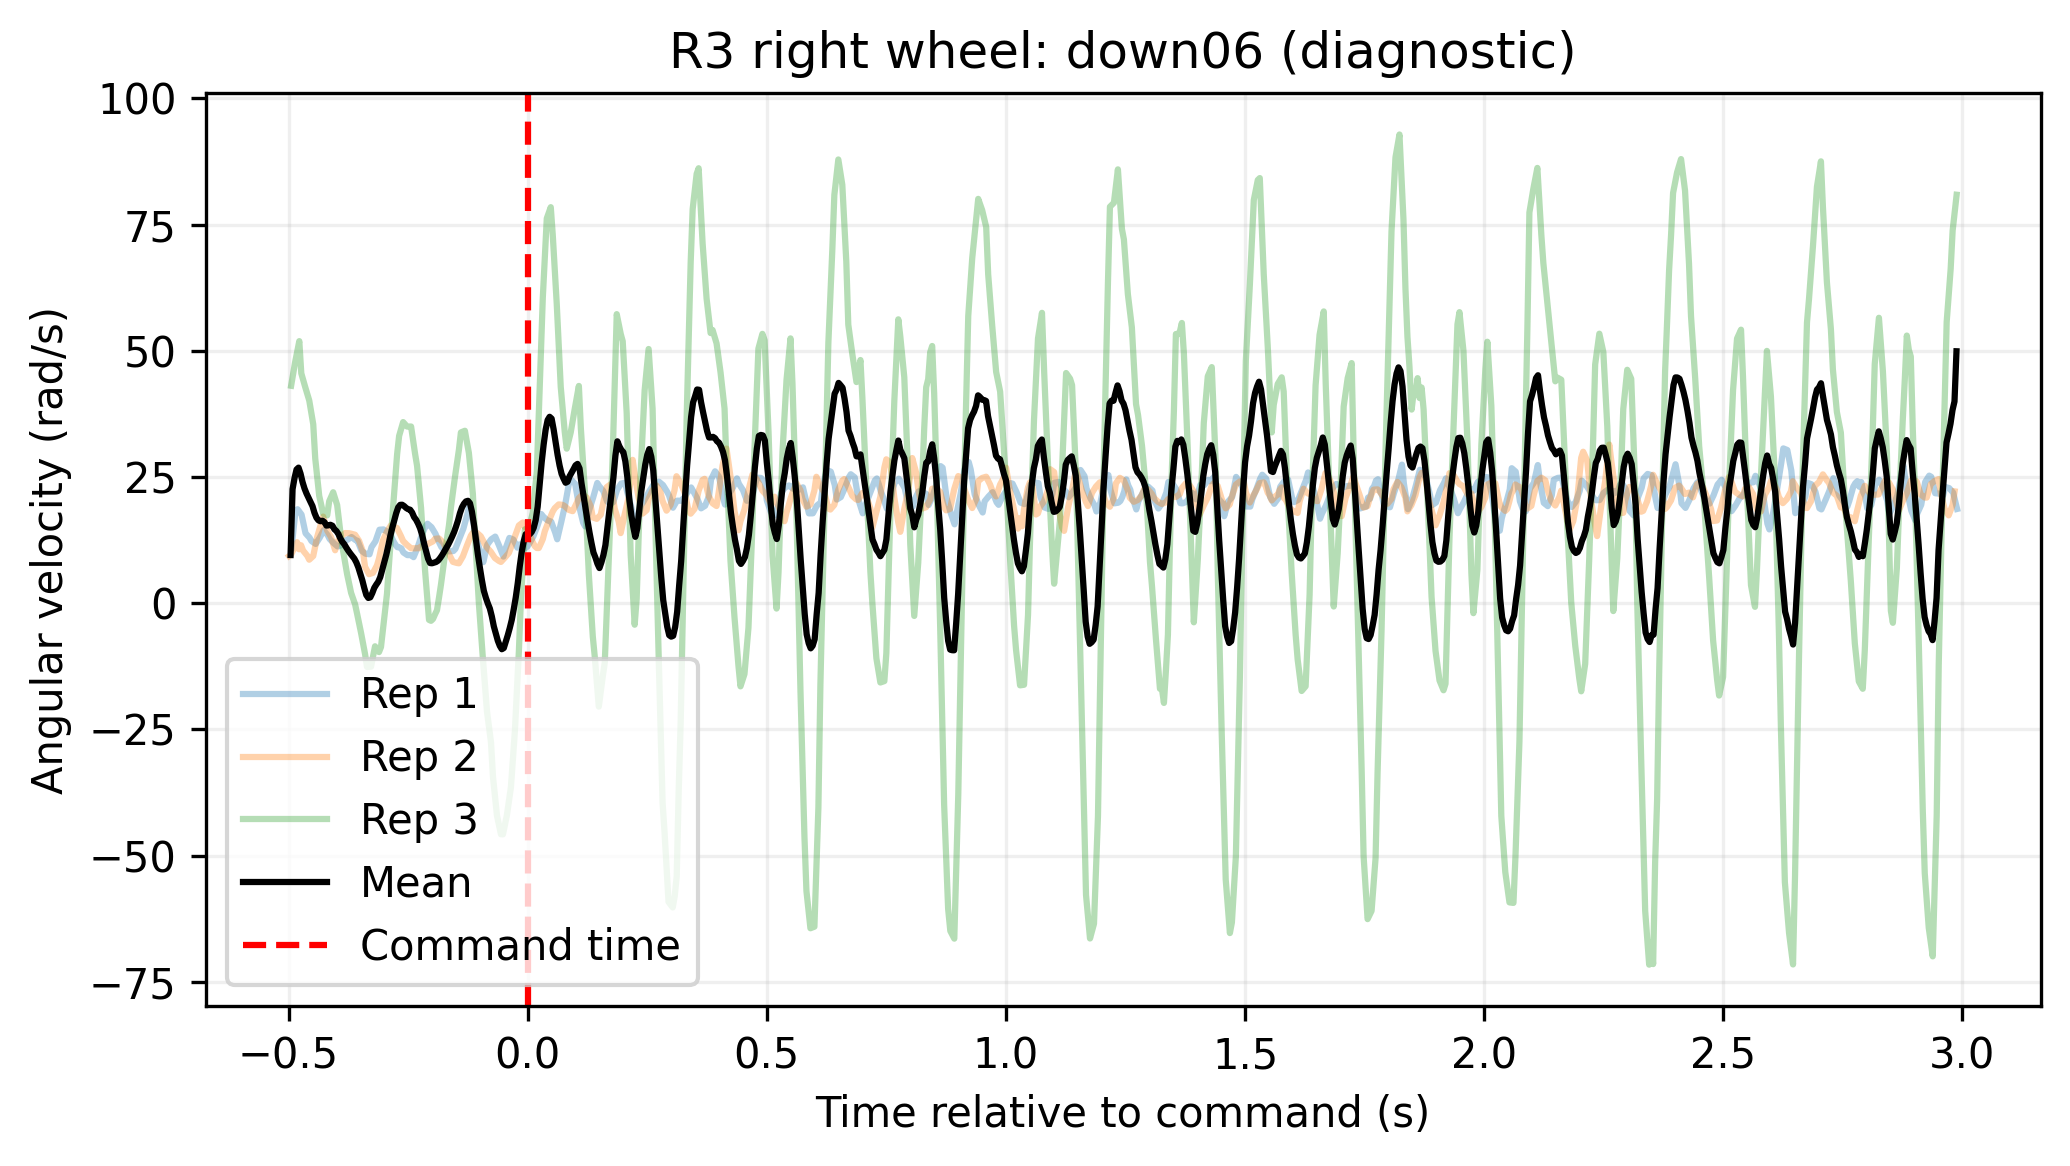
\includegraphics[width=0.85\linewidth,height=0.32\textheight,keepaspectratio]{R3_E2_down06_diagnostic.png}\caption{Right wheel, step from 1.0 to 0.6. Diagnostic plot; timing and tracking are not validated.}\end{figure}
\begin{figure}[H]\centering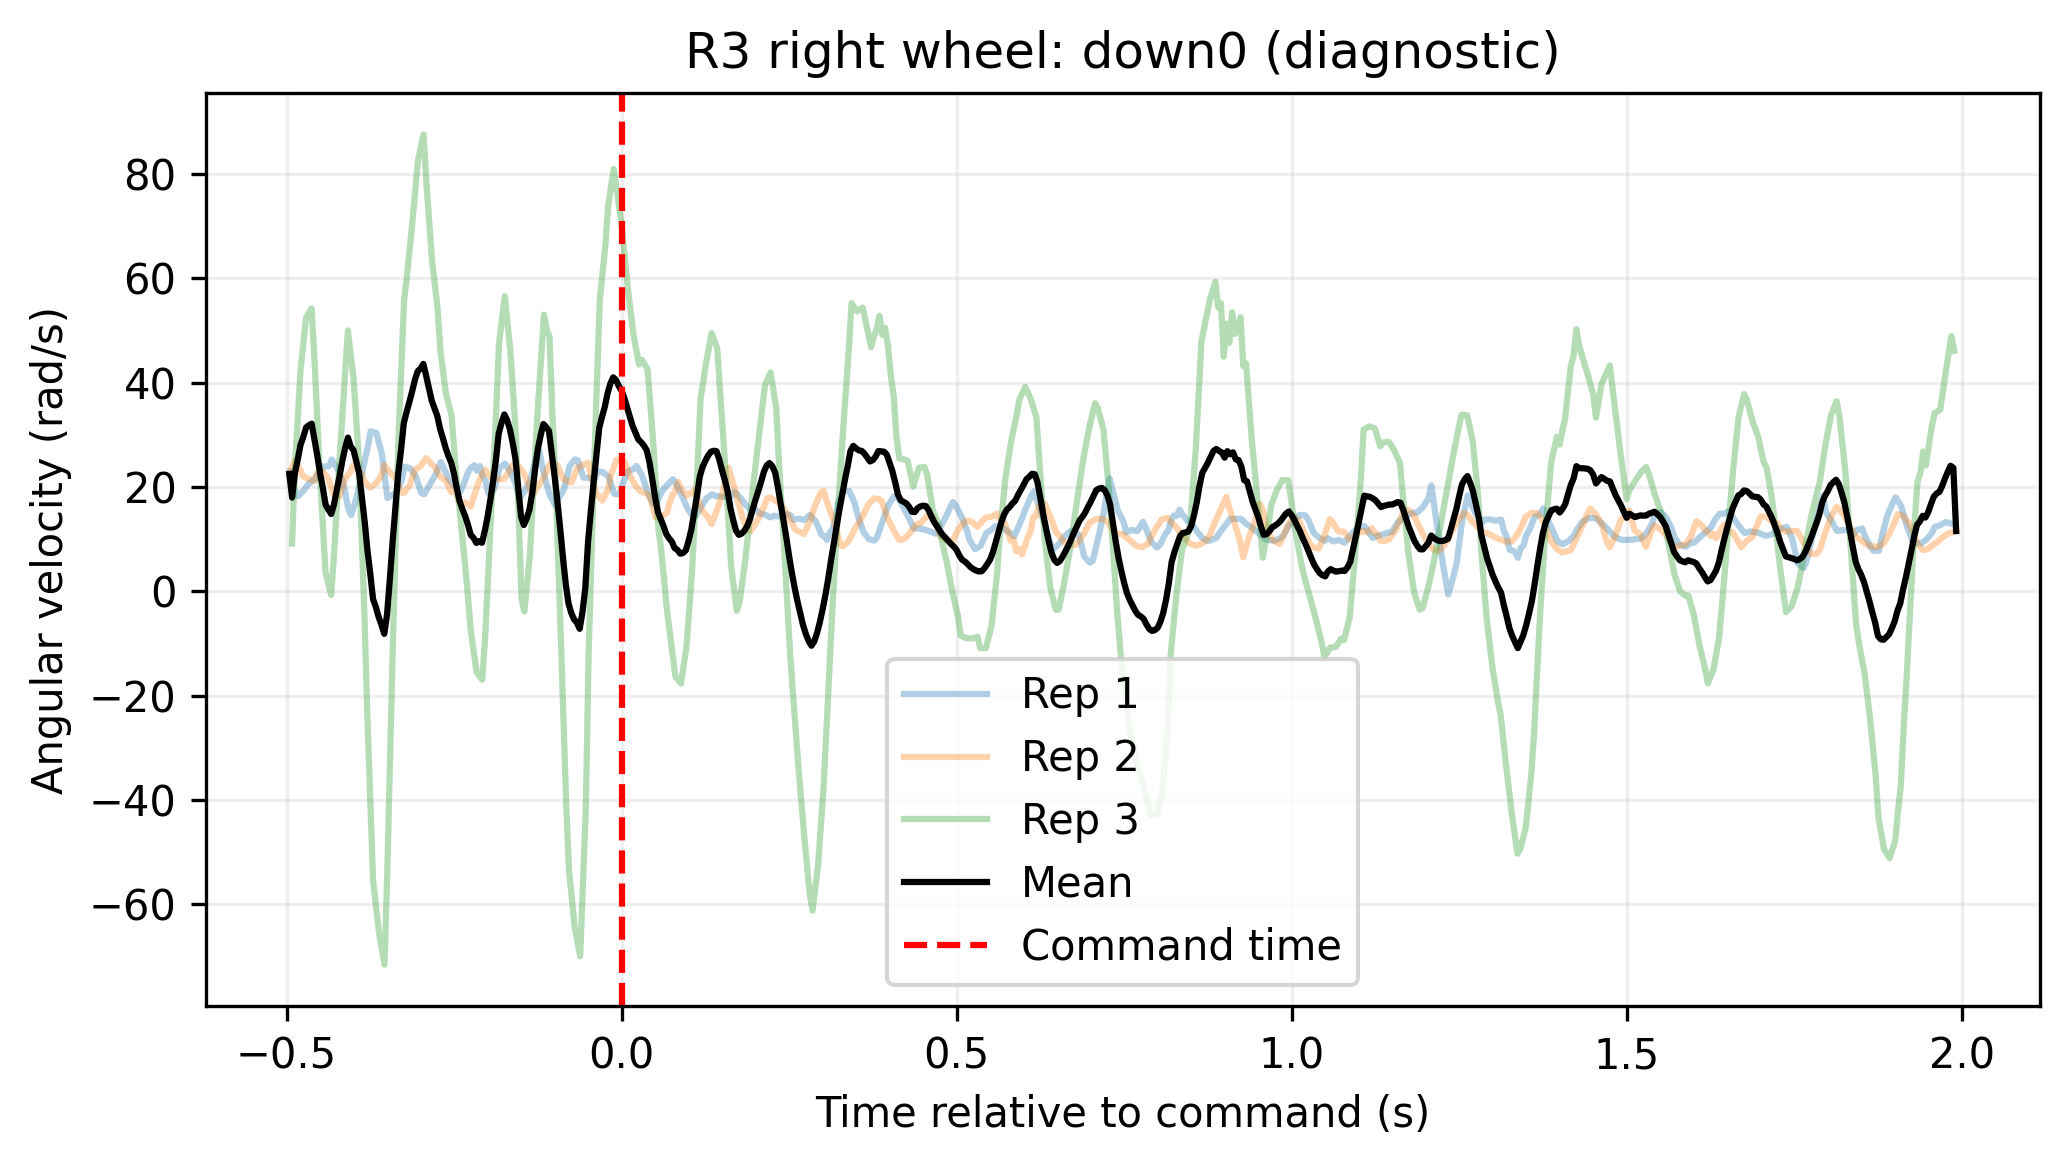
\includegraphics[width=0.85\linewidth,height=0.32\textheight,keepaspectratio]{R3_E2_down0_diagnostic.png}\caption{Right wheel, step from 0.6 to 0. Diagnostic plot; timing and tracking are not validated.}\end{figure}
\subsection{Hysteresis (4d, P3)}
The right-wheel increasing and decreasing duty branches differ, but the synchronization errors prevent a reliable hysteresis measurement. The left negative-duty sweep approached rest at magnitude 0.22, suggesting an apparent start--stop gap of 0.06. This is descriptive only. The right-wheel downward step from 1 to 0.6 showed an apparent increase in speed, and the final step to zero did not return to rest in the aligned endpoint means. These inconsistencies cannot establish physical asymmetry. Removing repetition 3 alone would not resolve the anomalous responses in the other repetitions.

\begin{figure}[H]\centering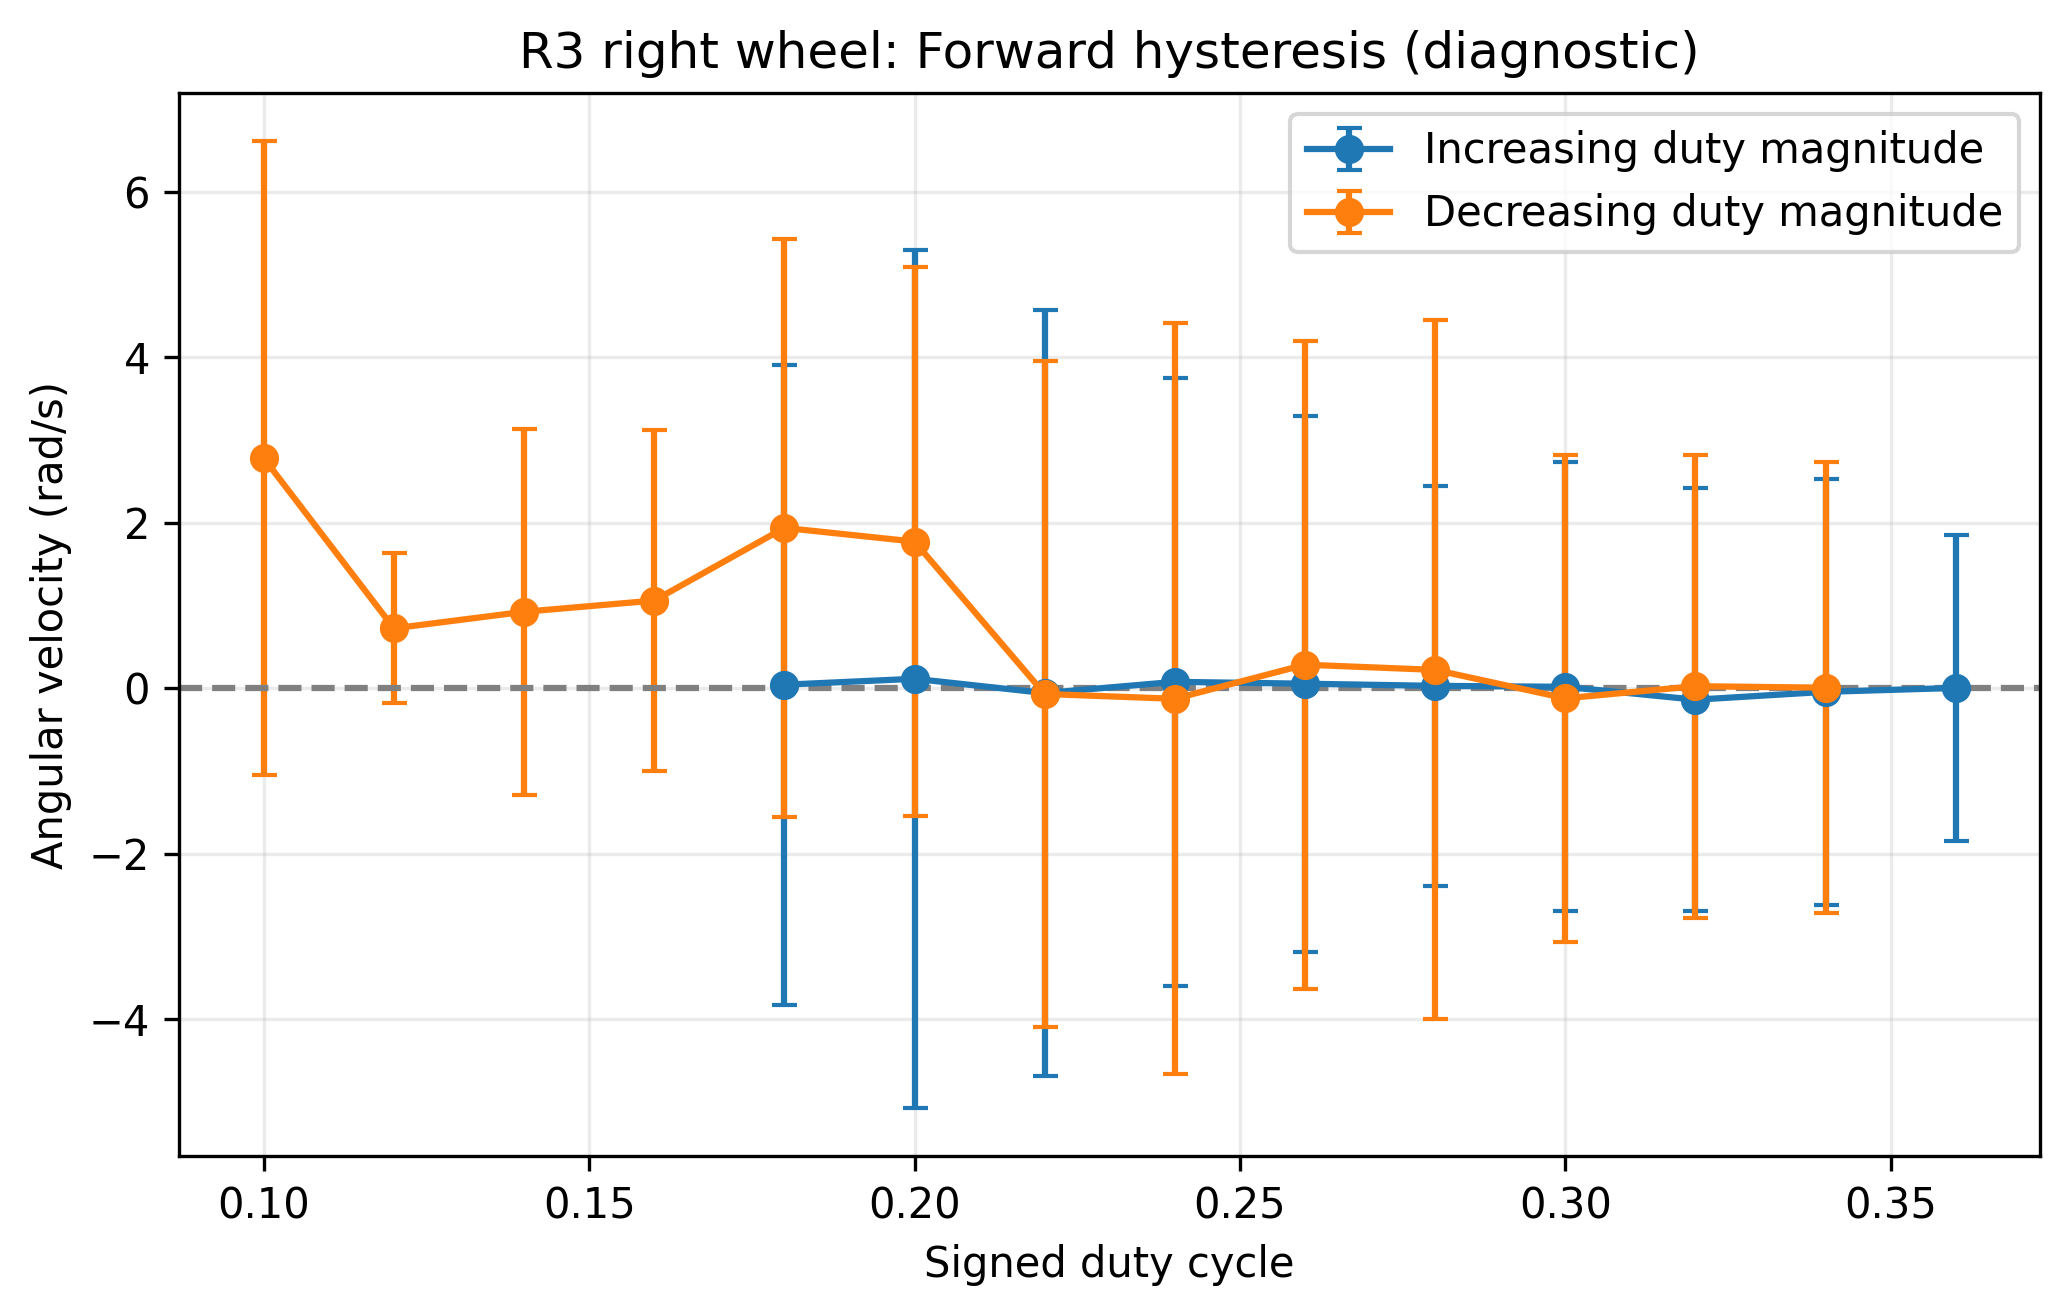
\includegraphics[width=0.85\linewidth,height=0.32\textheight,keepaspectratio]{R3_E1_Forward_hysteresis.png}\caption{Right wheel, positive-duty E1 branches. Diagnostic plot; timing and tracking are not validated.}\end{figure}
\begin{figure}[H]\centering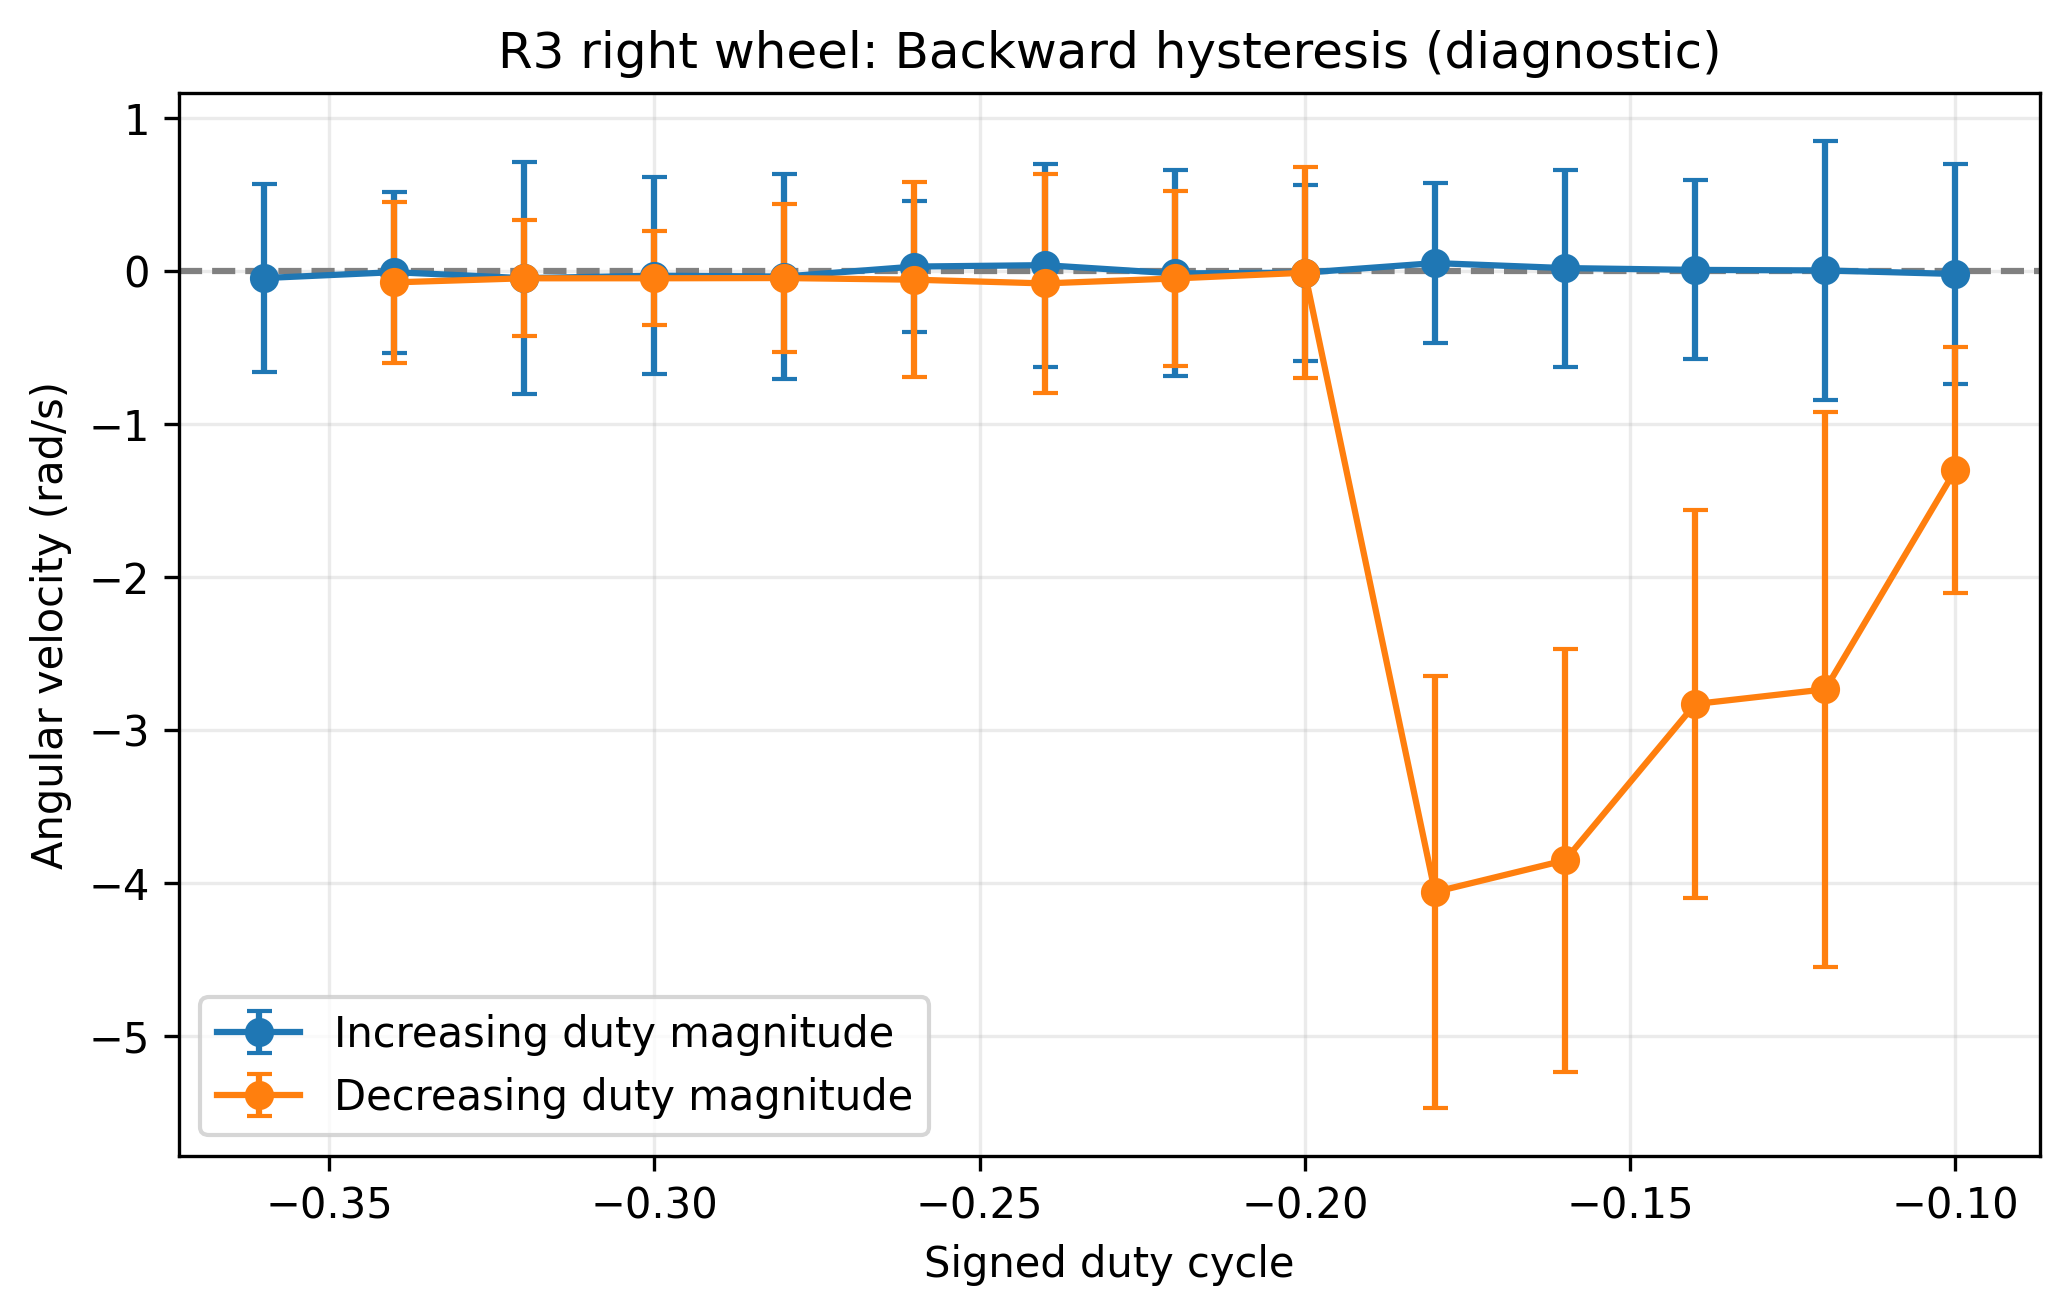
\includegraphics[width=0.85\linewidth,height=0.32\textheight,keepaspectratio]{R3_E1_Backward_hysteresis.png}\caption{Right wheel, negative-duty E1 branches. Diagnostic plot; timing and tracking are not validated.}\end{figure}
\section{Discussion}
The main limitation is measurement validity rather than the choice of model. Timing discrepancies can assign wheel motion to the wrong duty plateau, while marker-tracking errors can create large apparent velocities. These mechanisms are plausible explanations, not confirmed root causes. The missing left forward trial prevents a complete direction comparison. Missing manual wheel and marker radii prevent conversion to ground speed or slip. The actual frame rate differs from the nominal camera setting. A repeat experiment should verify LED visibility, timing agreement, marker continuity and stationary intervals before fitting models; both directions should be recorded. No raw measurements were altered to force agreement with the expected model.
\section{Conclusions}
The standard analysis could not produce validated motor parameters because the quality checks failed and the rest threshold prevented start-duty identification. Diagnostic plots suggest possible dead-zone and hysteresis behavior, but P1--P3 remain inconclusive. Reliable synchronization and tracking are required before using the identified dynamics for controller design.
\section*{Acknowledgements}
The course analysis pipeline and report template were provided by the course staff.
\section*{Contributions}
All seven authors contributed equally (one seventh each); author order does not indicate differences in contribution. CRediT roles are listed below.

\textbf{林芳亘:} Formal analysis, Visualization, Writing -- original draft, Writing -- review and editing, Project administration.

\textbf{施嘉韙, 彭俊恆, 高至言:} Methodology, Investigation, Software, Data curation, Writing -- review and editing.

\textbf{許芯瑀:} Formal analysis, Visualization, Writing -- original draft, Writing -- review and editing.

\textbf{楊承軒:} Methodology, Investigation, Software, Data curation, Writing -- review and editing, Project administration.

\textbf{簡妤安:} Validation, Formal analysis, Visualization, Writing -- review and editing.
\section*{AI use}
ChatGPT was used to assist with diagnostic code, interpretation of quality warnings, preparation of plots, and drafting and integrating this LaTeX report. The reported diagnostic results are not substitutes for validated measurements. Authors are responsible for reviewing the final submission.
\printbibliography
\end{document}
